\documentclass[12pt,a4paper]{article}
\usepackage[left=2.5cm,right=2.5cm,top=2.5cm,bottom=2.5cm]{geometry}
\usepackage[utf8]{inputenc}
\usepackage{amssymb, amsmath, amsthm}
\usepackage{graphics, graphicx}
\graphicspath{ {./2.5/} }
\pagestyle{empty}
\newtheorem{lemma}{Lemma}
\newtheorem{thm}{Theorem}

\begin{document}
\textbf{Chapter 2 solutions  \hfill Hanna Gábor}

\begin{enumerate}
  \item
    \textit{In $\epsilon$-greedy action selection, for the case of two actions and $\epsilon = 0.5$, what is the probability that the greedy action is selected?}

    $\mathbb{P}(\text{greedy action is selected}) = 0.5 + 0.5/2 = 0.75.$

  \item
    \textit{Bandit example. Consider a $k$-armed bandit problem with $k = 4$ actions, denoted $1$, $2$, $3$, and $4$. Consider applying to this problem a bandit algorithm using $\epsilon$-greedy action selection, sample-average action-value estimates, and initial estimates of $Q_1(a) = 0$, for all $a$. Suppose the initial sequence of actions and rewards is $A_1 = 1$, $R_1 = 1$, $A_2 = 2$, $R_2 = 1$, $A_3 = 2$, $R_3 = 2$, $A_4 = 2$,
    $R_4 = 2$, $A_5 = 3$, $R_5 = 0$. On some of these time steps the $\epsilon$ case may have occurred, causing an action to be selected at random. On which time steps did this definitely occur? On which time steps could this possibly have occurred?}

    Any action can be an exploratory move.

    What were the greedy options in different time steps?\\
    Step $1$: all actions have $0$ estimated values. Every action is a greedy choice.\\
    Step $2$: $Q_1(1) = 1$. The greedy choice now is $1$. $A_2 = 2$ must have been an\\ explorative move.\\
    Step $3$: $Q_2(2) = 1$. The greedy choice is either $1$ or $2$.\\
    Step $4$: $Q_3(2) = 1.5$. The greedy choice is $2$.\\
    Step $5$: $Q_4(2) = 1.67$. The greedy choice is $2$. $A_5 = 3$ must have been an explorative move.

    On time steps $2$ and $5$ a random action must have been selected.

 \item
    \textit{In the comparison shown in Figure 2.2, which method will perform best in
    the long run in terms of cumulative reward and probability of selecting the best action?
    How much better will it be? Express your answer quantitatively.}

    On the long run, the $\epsilon = 0.01$ method will perform the best in both sense.
    The non-greedy methods will eventually find the best action, but only choose it
    with probability $1 - \epsilon + 0.01 \epsilon $. In the $\epsilon = 0.01$ case this means the method
    chooses the best action with probability $0.991$, while in the $\epsilon = 0.1$ case,
    this probability is $0.91$.

\item
  \textit{If the step-size parameters, $\alpha_n$, are not constant, then the estimate $Q_n$ is
  a weighted average of previously received rewards with a weighting different from that
  given by (2.6). What is the weighting on each prior reward for the general case, analogous
  to (2.6), in terms of the sequence of step-size parameters?}

  \begin{align*}
  Q_{n + 1} = & Q_n + \alpha(R_n - Q_n) = \alpha_n R_n + (1 - \alpha_n)Q_n \\
  = & \alpha_n R_n + (1 - \alpha_n)(Q_{n - 1} + \alpha_{n - 1}(R_{n - 1} - Q_{n - 1})) = \dots \\
  = & \Big(\prod\limits_{j = 1}^n (1 - \alpha_j)\Big) Q_1 +
  \sum\limits_{i = 1}^n \Big(\prod\limits_{j = i + 1}^n (1 - \alpha_j) \Big)\alpha_i R_i \\
  \end{align*}

\item
  \textit{(programming) Design and conduct an experiment to demonstrate the
  difficulties that sample-average methods have for nonstationary problems. Use a modified
  version of the 10-armed testbed in which all the $q_*(a)$ start out equal and then take
  independent random walks (say by adding a normally distributed increment with mean
  zero and standard deviation 0.01 to all the $q_*(a)$ on each step). Prepare plots like
  Figure 2.2 for an action-value method using sample averages, incrementally computed,
  and another action-value method using a constant step-size parameter, $\alpha = 0.1$. Use
  $\epsilon = 0.1$ and longer runs, say of 10,000 steps.}

  {\centering
  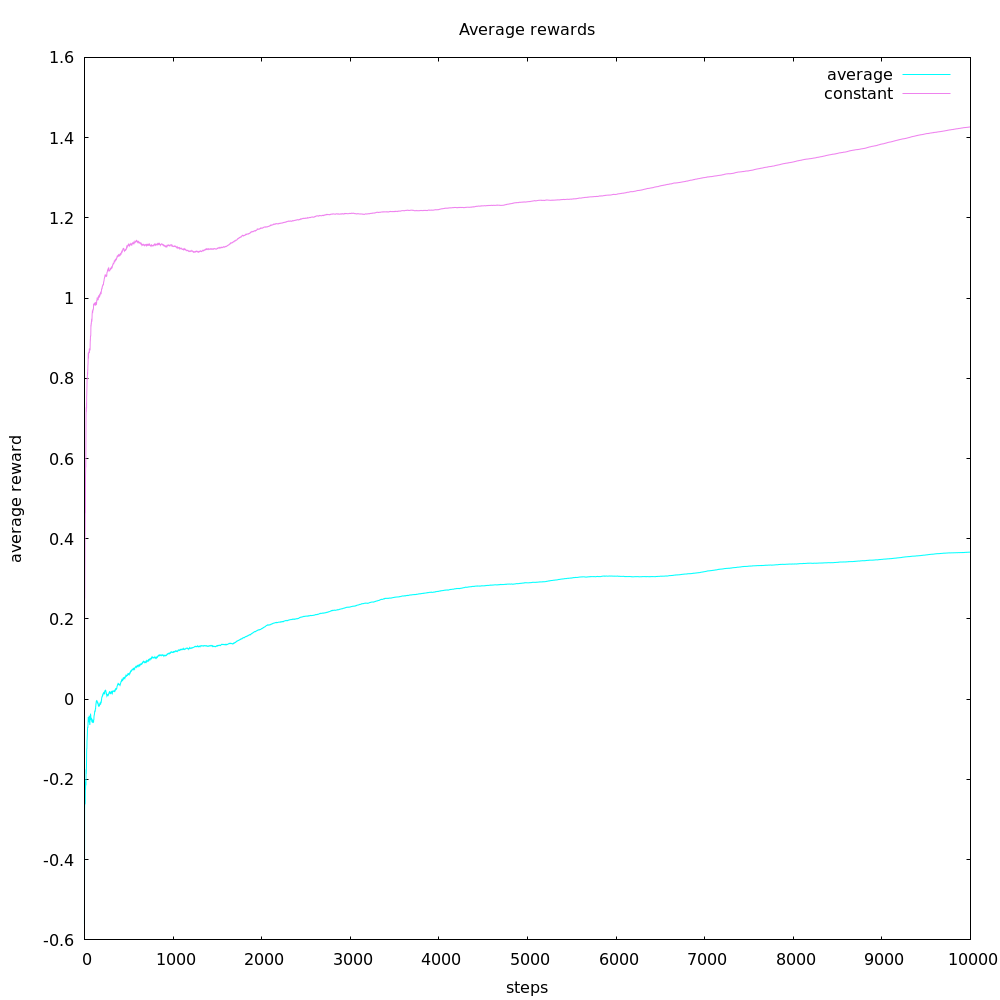
\includegraphics[scale=0.3]{average}

  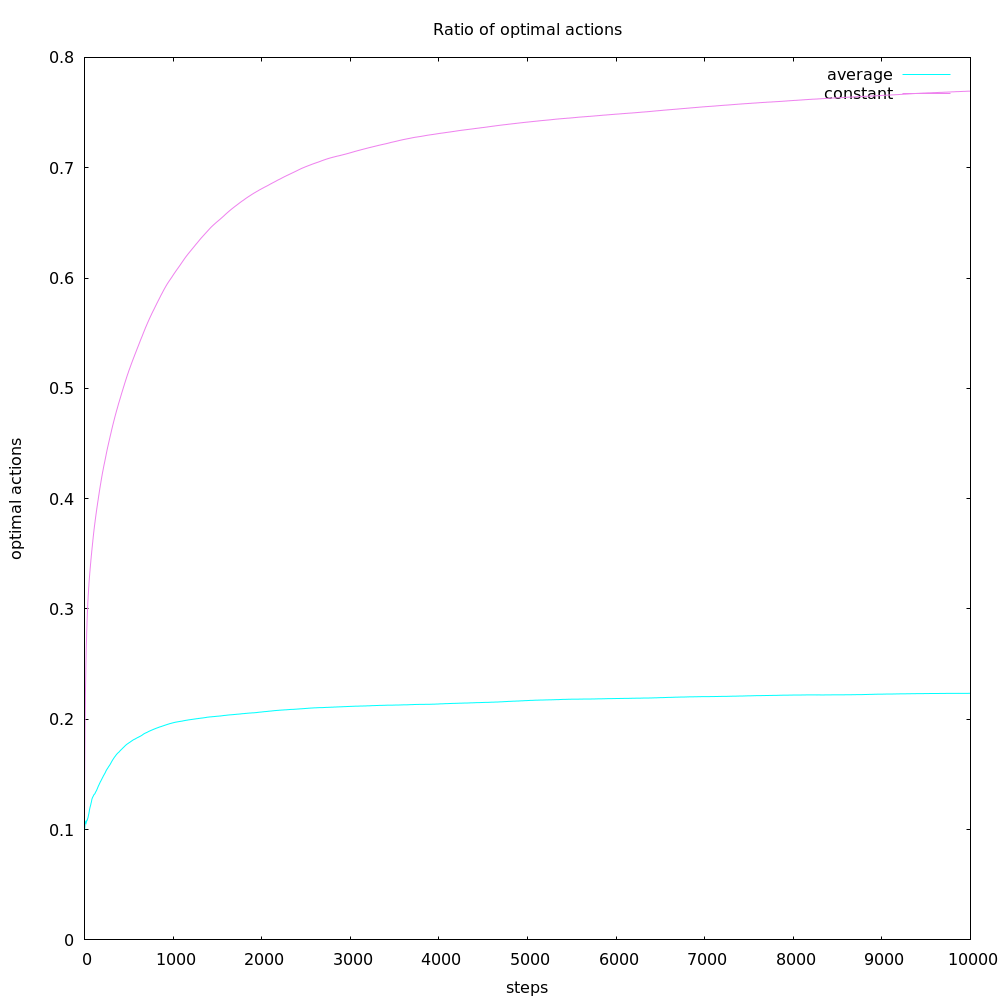
\includegraphics[scale=0.3]{optimal}
  }

\item
  \textit{Mysterious Spikes. The results shown in Figure 2.3 should be quite reliable
  because they are averages over 2000 individual, randomly chosen 10-armed bandit tasks.
  Why, then, are there oscillations and spikes in the early part of the curve for
  the optimistic method? In other words, what might make this method
  perform particularly better or worse, on average, on particular early steps?}

  With very high probability, the first $10$ choices will cover all the possible actions
  once. After the $10^th$ action, we have a an estimation of the action values based
  on the 


\end{enumerate}
\end{document}
